\documentclass[a4paper,UKenglish,cleveref,autoref,thm-restate]{lipics-v2021}

%% Bibliography style
\bibliographystyle{plainurl}

\usepackage{amsmath,amssymb}
\usepackage{booktabs}
\usepackage{algorithm}
\usepackage{algpseudocode}
\usepackage{tikz}
\usepackage{pgfplots}
\usepackage{pgfplotstable}
\pgfplotsset{compat=1.18}
\usetikzlibrary{positioning,arrows.meta,patterns,calc,decorations.pathreplacing,pgfplots.fillbetween}

% Path to root directory
\newcommand{\rootdir}{..}
\newcommand{\figdir}{../figures}

% Cross-reference macros (SEA uses cleveref, override for compatibility with shared sections)
\newcommand{\figref}[1]{\cref{#1}}
\newcommand{\tblref}[1]{\cref{#1}}
\newcommand{\secref}[1]{\cref{#1}}
\newcommand{\thmref}[1]{\cref{#1}}
\newcommand{\lemref}[1]{\cref{#1}}
\newcommand{\defref}[1]{\cref{#1}}
\newcommand{\appref}[1]{\cref{#1}}
\newcommand{\algoref}[1]{~\cref{#1}}

%% Title information
\title{DeltaSort: Incremental sorting of arrays with known updates}

%% Author information (anonymized for double-blind review)
\author{Anonymous Author(s)}{Affiliation withheld for review}{}{}{}

\authorrunning{Anonymous}

\Copyright{Anonymous Author(s)}

%% ACM Computing Classification System (CCS)
\ccsdesc[500]{Theory of computation~Sorting and searching}
\ccsdesc[300]{Theory of computation~Data structures design and analysis}

\keywords{Incremental sorting, Sorting algorithms, Array maintenance, Experimental algorithmics}

%% Data availability statement
\supplement{Source code and benchmark data are available at \url{https://www.dropbox.com/scl/fo/bi7mkpe94llo1bon2o7t3/AN0SegS5b-TCABRJErJTA9g?rlkey=ealdnsqsjkwfb4h1cbb4kyzvj&st=qjrh9owg&dl=0} (anonymized for review). Benchmark results are reproducible using the instructions in the repository README.}

\nolinenumbers

\begin{document}

\maketitle
\begin{abstract}
% Abstract
Sorting values or records is a fundamental operation in many systems. When records need to be read in a particular order, sorting at read time incurs repeated $O(n \log n)$ cost and can become a bottleneck in read-heavy workloads. A common solution is to maintain a derived sorted read-replica that is kept updated asynchronously as the underlying data changes. For updating read-replicas that are stored as arrays, existing approaches rely either on full re-sorting or on incremental techniques such as repeated binary insertion, which incurs high data movement, or merge-based strategies, which require linear auxiliary space. In this paper, we study incremental sorting under a model in which the sorting routine is explicitly informed of the indices of elements updated since the previous sort—a setting that naturally arises in systems that track update deltas. Under this model, we present \emph{DeltaSort}, a new algorithm for incremental sorting that occupies an intermediate point in the time-space trade-off spectrum. We provide theoretical analysis and experimental evidence showing that, for random update distributions, \emph{DeltaSort} achieves lower execution time than insertion-based incremental sorting while using substantially less auxiliary space than merge-based approaches.
\end{abstract}

%==============================================================================
\section{Introduction}
\label{sec:introduction}
%==============================================================================

Sorting is among the most heavily optimized primitives in modern systems, backed by decades of deep research. Standard library implementations---TimSort~\cite{timsort}, Introsort~\cite{musser1997introspective}, and DriftSort~\cite{driftsort} deliver excellent performance for general inputs by exploiting existing order, cache locality, and adaptive strategies. However, these algorithms operate under a \emph{blind} model: they discover structure dynamically rather than being explicitly informed about which values have been updated since the previous sort. While this model is more general and makes things straightforward for the caller, it also misses opportunities for optimization when such information is available. Modern systems often maintain metadata about updated records as part of their execution pipeline~\cite{kleppmann2017cdc}, making it possible to expose this information to lower-level sorting primitives. In the absence of a primitive that can accept this as a first-class input, they must either perform a full re-sort or use standard insertion-based or merge-based incremental techniques.

As an example, consider a modern client application that needs to display a large dynamic sorted list of items (e.g. task management applications or interactive dashboards). Modern applications have tight latency budgets for main-thread execution, beyond which users perceive the interface as unresponsive \cite{webdev_inp,card1983psychology}. As a result, UI frameworks commonly encourage memoization to avoid repeated recomputation of expensive derived values such as sorted views \cite{react_usememo}. However, such memoization is typically coarse-grained: cached results are invalidated whenever dependencies change, without exploiting knowledge of which positions were updated \cite{acar2006self}. Consequently, repeated full re-sorting can occupy the main thread long enough to exceed responsiveness budgets, leading to janky user experiences \cite{webdev_inp,googleRAIL}. If a sorting primitive could be informed of which elements were updated, it could potentially restore sorted order more efficiently than a full re-sort, enabling more responsive user interfaces.

Once the indices of the updates are known, how do we exploit this extra information to restore order more efficiently than performing a full re-sort? While similar questions arise for a variety of ordered data structures (e.g. B-Trees, heaps and BSTs), in this paper we deliberately focus on \textbf{arrays}, which provide a contiguous memory layout. This choice is intentional: arrays remain the dominant representation for sorted data in performance-critical systems because they offer superior cache locality and enable SIMD/vectorized processing~\cite{hennessy2017computer}—benefits that pointer-based structures fundamentally cannot provide. As a result, many systems prefer to preserve array layouts even when updates are frequent, rather than switching to fully dynamic structures~\cite{drepper2007memory,abadi2008columnstores,boncz2005monetdb}. This also allows us to cleanly isolate the algorithmic consequences of exposing update indices to the sorting routine and study the resulting trade-offs in a concrete setting.

Existing approaches for incrementally sorting arrays force a choice between two extremes:
\begin{enumerate}
  \item Binary-Insertion-Sort (\textbf{BIS}): Collect all updated values from the array and insert them back one by one using binary search. This approach uses $O(1)$ extra space but incurs $O(k n)$ data movement for $k$ updates in an array of size $n$, making it suitable only for very small update batches. This is the \emph{space-efficient but time-inefficient}  option on the trade-off frontier.
  \item Extract–Sort–Merge (\textbf{ESM}): Extract all updated values into a separate array, sort them using an efficient $O(k \log k)$ algorithm, and then merge them back into the original array. This approach uses $O(k \log k + n)$ time, but $O(n)$ extra space, even for small $k$, making it suitable only for larger update batches. This is the \emph{time-efficient but space-inefficient} option on the trade-off frontier.
\end{enumerate}

This raises the question: are there other algorithms that offer \emph{intermediate} trade-offs? To our knowledge, no prior work exploits knowledge of updated indices to achieve a better time-space trade-off than the two extremes listed above. In this paper, we fill that gap. Specifically, this paper makes the following contributions:

\begin{enumerate}
  \item \textbf{Update-aware sorting model:} We formulate a sorting model in which the sorting routine is explicitly informed of the updated indices since the previous sort. Under this model, BIS and ESM serve as the baseline algorithms because they can naturally exploit knowledge of which indices have been updated. 

  \item \textbf{DeltaSort algorithm:} We present \emph{DeltaSort}, an update-aware sorting algorithm, which offers distinct trade-offs (\figref{tab:incremental-sorting-algorithms}) as compared to existing approaches. We prove its correctness using loop invariants and illustrate its operation with examples.
  
  \item \textbf{Theoretical analysis:} Under a random bounded-range update model, we show that DeltaSort achieves $O(k \log n + n \sqrt{k})$ amortized time complexity while needing only $O(k)$ auxiliary space.
  
  \item \textbf{Experimental validation:} We implement DeltaSort in Rust and benchmark it against BIS, ESM, and full re-sorting on synthetic datasets. Our results show that DeltaSort is consistently faster than BIS in our evaluation and provides a space-efficient alternative to ESM across a wide range of update sizes.
\end{enumerate}

Although we study DeltaSort as a standalone algorithm for clarity, for practical application, it is best viewed as a \emph{building block} in a hybrid strategy that combines multiple update-aware techniques.
\begin{table}
\centering
\caption{Algorithms for update-aware sorting}
\label{tab:incremental-sorting-algorithms}
\begin{tabular}{l c c}
\toprule
Algorithm & Time (Expected / Worst) & Space \\
\midrule
Binary-Insertion-Sort$^{\dagger}$ & $O(kn)$ & $O(1)$ \\
Extract–Sort–Merge$^{*}$$^{\dagger}$ & $O(k \log k + n)$ & $O(n)$ \\
\textbf{DeltaSort}$^{*}$ & $O(n\sqrt{k})\,/\,O(kn)$ & $O(k)$ \\
\bottomrule
\end{tabular}

\vspace{0.3em}
{$n$ = array size, $k$ = number of updates}

\small $^{*}$These use a full sort primitive internally assumed to run in $O(k \log k)$ time and $\le O(k)$ space.

\small $^{\dagger}$These have the same expected and worst case time complexity.
\end{table}


%==============================================================================
\section{Related Work}
\label{sec:related}
%==============================================================================

Adaptive sorting algorithms exploit existing order in the input to improve performance on nearly sorted data. TimSort~\cite{timsort} and natural merge sort~\cite{knuth1998art} dynamically identify monotonic runs and merge them efficiently, while a substantial body of work formalizes measures of presortedness and analyzes sorting complexity as a function of these measures rather than input size alone~\cite{mannila1985measures}. These approaches, however, assume no explicit knowledge of which values have been updated.

Prior work has also used the term \emph{incremental sorting} in different contexts. Aydin and Anderson~\cite{7184878} study incremental sorting of large, dynamic data sets in distributed systems, where new records are continuously appended and sorted along multiple dimensions using batch processing frameworks such as Hadoop. Their focus is on scalable index construction and query-time performance rather than on fixing a sorted array after in-place updates. As a result, their approach does not consider the cost of local data movement, nor does it exploit explicit knowledge of which array positions have been updated.

Closer to the algorithmic literature, Paredes and Navarro~\cite{paredes2006optimal} present an optimal online algorithm for incremental \emph{selection}, which outputs the next smallest value of a set on demand. While related in spirit, their work addresses partial sorting and selection rather than maintaining a fully sorted array under updates.

A separate line of work studies incremental computation and view maintenance in database and streaming systems, where updates to input data are propagated to derived results using explicit delta representations~\cite{gupta1995maintenance, nikolic2014incremental, akidau2015dataflow}. These techniques focus on maintaining query results, aggregates, and materialized views, and operate at the level of relational or dataflow operators rather than array-based sorting primitives. They treat deltas as first-class citizens and demonstrate the practical value of update-aware computation. However, they do not specifically address the problem of incrementally sorting arrays, which is a much more specialized, lower-level problem.

Dynamic data structures offer a different trade-off. Self-balancing trees such as AVL trees~\cite{avl1962}, red--black trees~\cite{guibas1978dichromatic}, B-trees~\cite{bayer1972organization}, and skip lists~\cite{pugh1990skip} support efficient ordered updates with logarithmic cost, but abandon contiguous array layout and its associated advantages.

In contrast, this work focuses on a more specialized but fundamental problem: maintaining sorted order in contiguous arrays after a batch of in-place updates, under the assumption that the indices of updated values are explicitly available. This setting is not addressed by adaptive sorting algorithms, system-level incremental indexing techniques, or selection-based incremental algorithms. \emph{DeltaSort} operates as a low-level sorting primitive that complements higher-level incremental systems, while preserving the cache locality and simplicity of array-based layouts.
%==============================================================================
\section{Problem Model}
\label{sec:model}
%==============================================================================

\begin{definition}[Update-Aware Sorting]
\label{def:problem}

Let $A[0..n-1]$ be an array of size $n$ that is initially sorted according to a strict weak ordering induced by a comparator $\texttt{cmp}$. Let $U \subseteq \{0,\dots,n-1\}$ be a set of $k$ distinct indices such that the values at indices in $U$ may have been arbitrarily updated\footnote{This model can be easily extended to insertions and deletions as well. Insertions can be handled by appending the new value to the end of the array and adding $n$ to $U$. Deletions can be reduced to updates by assigning a sentinel value larger than all existing values and truncating the array after sorting.}, while values at all other indices remain unchanged. The \emph{update-aware sorting problem} is to restore the global sorted order of $A$ with respect to $\texttt{cmp}$, given explicit knowledge of the update set $U$.
\end{definition}

The sorting primitive in this model requires the caller to store the $k$ updated indices incurring an extra $O(k)$ space overhead compared to full re-sorting. This overhead is modest and aligns with how updates are applied in practice: locating and updating a value already requires identifying its position, and recording that position incurs only constant additional cost per update. In contrast, avoiding this bookkeeping typically forces the system to fall back to either full re-sorting, which incurs $O(n \log n)$ time cost per update, or BIS, which incurs $O(n)$ data movement cost per update. Modern streaming and stateful processing systems~\cite{kleppmann2017ddiamodernsystems} routinely track update deltas as part of their execution pipelines, making the update-aware model a natural and practically useful abstraction.
% Figure: DeltaSort algorithm example
\begin{figure}[t]
\centering
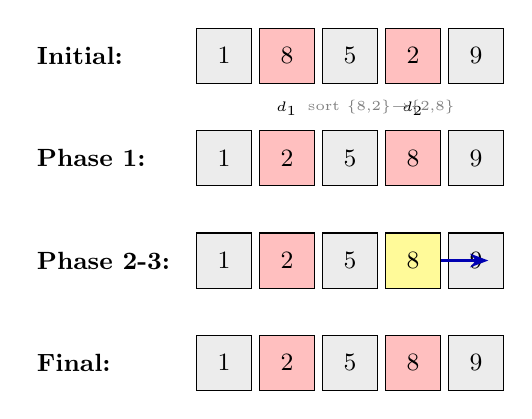
\begin{tikzpicture}[
    element/.style={minimum width=0.7cm, minimum height=0.7cm, draw, font=\small},
    dirty/.style={element, fill=red!25},
    clean/.style={element, fill=gray!15},
    arrow/.style={-{Stealth}, thick, blue!70!black},
    phase/.style={font=\small\bfseries, anchor=west}
]

% Phase labels
\node[phase] at (-2.5, 0) {Initial:};
\node[phase] at (-2.5, -1.3) {Phase 1:};
\node[phase] at (-2.5, -2.6) {Phase 2-3:};
\node[phase] at (-2.5, -3.9) {Final:};

% Initial: sorted array [1,3,5,7,9] with dirty at 1,3 getting values 8,2
\node[clean] (i0) at (0*0.8, 0) {1};
\node[dirty] (i1) at (1*0.8, 0) {8};
\node[clean] (i2) at (2*0.8, 0) {5};
\node[dirty] (i3) at (3*0.8, 0) {2};
\node[clean] (i4) at (4*0.8, 0) {9};
\node[font=\tiny, below=0.1cm of i1] {$d_1$};
\node[font=\tiny, below=0.1cm of i3] {$d_2$};

% After Phase 1: sort {8,2} -> {2,8}, write to {1,3}
\node[clean] (p10) at (0*0.8, -1.3) {1};
\node[dirty] (p11) at (1*0.8, -1.3) {2};
\node[clean] (p12) at (2*0.8, -1.3) {5};
\node[dirty] (p13) at (3*0.8, -1.3) {8};
\node[clean] (p14) at (4*0.8, -1.3) {9};
\node[font=\tiny, text=gray] at (2.5*0.8, -0.65) {sort \{8,2\}$\to$\{2,8\}};

% After Phase 2-3: 8 needs to move right
\node[clean] (p20) at (0*0.8, -2.6) {1};
\node[dirty] (p21) at (1*0.8, -2.6) {2};
\node[clean] (p22) at (2*0.8, -2.6) {5};
\node[dirty,fill=yellow!40] (p23) at (3*0.8, -2.6) {8};
\node[clean] (p24) at (4*0.8, -2.6) {9};
\draw[arrow] (p23.east) to[out=0,in=180] ++(0.6,0);

% Final
\node[clean] (f0) at (0*0.8, -3.9) {1};
\node[dirty] (f1) at (1*0.8, -3.9) {2};
\node[clean] (f2) at (2*0.8, -3.9) {5};
\node[dirty] (f3) at (3*0.8, -3.9) {8};
\node[clean] (f4) at (4*0.8, -3.9) {9};

\end{tikzpicture}
\caption{DeltaSort example. Dirty indices $\{1,3\}$ with values $\{8,2\}$. Phase 1 sorts
dirty values to $\{2,8\}$ and writes back, establishing monotonicity for bounded search.}
\label{fig:algorithm}
\end{figure}

%==============================================================================
\section{Experimental Evaluation}
\label{sec:experiments}
%==============================================================================

All experiments \footnote{Along with experiments, we also validated correctness by an extensive set of randomized tests~\cite{deltasort-repo} across various scales of $n$ and full range of $k$.} are conducted on Rust implementations of each algorithm on synthetic datasets of user objects (name, age, country), and executed on an Apple M3 Pro. We use Rust as the primary evaluation language due to its predictable performance characteristics \footnote{In contrast, managed execution environments like JavaScript on V8 have various factors like garbage collection, non-contiguous memory layouts~\cite{v8elementskinds} etc. that impact the underlying cost model.}. Execution times are measured after sufficient warm-up iterations to account for caching and allocator effects. Each reported data point corresponds to the mean over repeated runs, with a 95\% confidence interval of at most $5\%$. The benchmarking routines are provided in the repository for reproducibility~\cite{deltasort-repo}. We used fully random update distributions, which provide no favorable structure to any particular algorithm. We evaluated following algorithms:

\begin{itemize}
  \item \textbf{NativeSort}: Rust's \texttt{sort\_by} implementation based on PDQSort~\cite{peters2021pdqsort}, representing full re-sorting of the array. NativeSort serves as a critical baseline to identify the crossover threshold $k_c$ for each update-aware algorithm beyond which full re-sorting becomes preferable.

  \item \textbf{Binary-Insertion-Sort (BIS)} and \textbf{Extract--Sort--Merge (ESM)}: standard update-aware sorting algorithms that represent distinct time--space trade-offs, as described in \secref{sec:introduction}.

  \item \textbf{DeltaSort}: our proposed update-aware sorting algorithm, as described in \secref{sec:algorithm}.
\end{itemize}

\begin{table}[t]
\centering
\caption{Algorithm complexity comparison}
\label{tab:complexity}
\begin{tabular}{l c c c c}
\toprule
Algorithm & Comparisons (C) & Movement (M) & Space (S) & Time (C + M) \\
\midrule
FullSort$^{*}$ $(\texttt{sort\_by})$ & $O(n \log n)$ & - & - & $O(n \log n)$ \\
BIS & $O(k \log n)$ & $O(kn)$ & $O(1)$ & $O(kn)$ \\
ESM & $O(k \log k + n)$ & $O(n)$ & $O(n)$ & $O(k \log k + n)$ \\
\textbf{DeltaSort} & $O(k \log n)$ & $O(n\sqrt{k})$ & $O(k)$ & $O(k \log n + n \sqrt k)$$^{\dagger}$ \\
\bottomrule
\end{tabular}

\vspace{0.3em}
{\small $^{*}$Not update-aware; hence complexity is a function of only $n$. The exact movement and space complexity are implementation-dependent and not required for the present discussion.}


{\small $^{\dagger}$Expected. Worst-case time is $O(kn)$}
\end{table}

\subsection{Execution Time}

\figref{fig:rust-execution-time} shows execution time (in \textmu s) for $n = 100$K values as a function of the number of updated values $k$ on a log--log scale. We use a log--log scale to highlight interesting behavior at lower ranges of $k$, which is the most practically relevant regime. As $k$ increases, all update-aware algorithms eventually lose to NativeSort (\emph{crossover threshold}), as the overhead of processing updates begins to overshadow any benefit from harnessing the presortedness.

% Figure: All algorithms comparison (log-log scale)
\begin{figure}[H]
\centering
\begin{tikzpicture}
\begin{axis}[
    width=0.8\textwidth,
    height=5cm,
    xlabel={Number of updated values ($k$)},
    ylabel={Execution time (\textmu s)},
    xmode=log,
    ymode=log,
    log basis x=10,
    log basis y=10,
    xmin=1, xmax=100000,
    ymin=5, ymax=100000,
    xtick={1, 10, 100, 1000, 10000, 100000},
    xticklabels={1, 10 (0.01\%), 100 (0.1\%), 1K (1\%), 10K (10\%), 100K},
    legend pos=south east,
    legend style={font=\small, fill=white, fill opacity=0.95, draw=gray!50},
    grid=major,
    major grid style={line width=0.3pt, draw=gray!30},
    tick label style={font=\small},
    label style={font=\small},
]

% FullSort
\addplot[color=gray!70, mark=square*, thick, mark size=2pt] 
    table[col sep=comma, x=k, y=native] {\rootdir/figures/js/execution-time.csv};

% Binary Insertion
\addplot[color=orange!80, mark=triangle*, thick, mark size=2pt] 
    table[col sep=comma, x=k, y=bis] {\rootdir/figures/js/execution-time.csv};
% Extract-Sort-Merge
\addplot[color=purple!70, mark=diamond*, thick, mark size=2pt] 
    table[col sep=comma, x=k, y=esm] {\rootdir/figures/js/execution-time.csv};

% DeltaSort (emphasized)
\addplot[color=green!70!black, mark=*, thick, mark size=2.5pt, line width=1.5pt] 
    table[col sep=comma, x=k, y=deltasort] {\rootdir/figures/js/execution-time.csv};

\legend{FullSort, BIS, ESM, \textbf{DeltaSort}}
\end{axis}
\end{tikzpicture}
\caption{Execution time comparison for JavaScript implementations for $n = 100$K (log-log scale).}
\label{fig:js-execution-time}
\end{figure}


Several observations emerge from the execution-time profile:

\begin{enumerate}
  \item The asymptotic behavior for each algorithm aligns with theoretical expectations. BIS exhibits superlinear growth consistent with its $O(kn)$ movement cost, while ESM and DeltaSort converge toward $O(n \log n)$ behavior as $k$ approaches $n$.
  \item \textbf{DeltaSort is the fastest baseline for} $k \lesssim 1\%$. It uses more auxiliary space than BIS ($O(k)$ vs $O(1)$) but substantially less than ESM ($O(k)$ vs $O(n)$). This regime is small in absolute terms, but aligns well with practical workloads where deltas are usually a small percentage of the full dataset.

  \item ESM is the fastest baseline across most of the intermediate range ($1\% \lesssim k \lesssim 80\%$). Although, its performance comes at the cost of $O(n)$ auxiliary space. DeltaSort provides a more space-efficient alternative to ESM for $k \lesssim 30\%$, albeit with higher execution time.
\end{enumerate}

These observations suggest that, much like hybrid blind sorting algorithms (e.g., TimSort~\cite{timsort}, PDQSort~\cite{peters2021pdqsort}), it would be beneficial to construct \emph{hybrid update-aware} strategies that are adaptive. As an example, for the Rust implementation evaluated here, a balanced strategy for an environment that requires fast execution without excessive space usage would be:

\begin{center}
  Use DeltaSort for $k \lesssim 10\%$, ESM for $10\% \lesssim k \lesssim 80\%$, and NativeSort for $k \gtrsim 80\%$.
\end{center}

The optimal crossover thresholds for a scenario would depend on several factors like memory availability, distribution of update sizes etc. The key takeaway is that DeltaSort occupies a distinct and practically relevant point in the time--space trade-off spectrum for update-aware sorting.

\subsection{Comparison Count}
Comparator cost is another factor that influences performance and varies widely across scenarios. For our evaluation, we picked a multi-key comparator that is a realistic proxy for practical use cases. Our experiments show that DeltaSort’s comparator invocation count closely tracks that of Binary-Insertion-Sort, consistent with the $O(k \log n)$ theoretical bound. As a result, when comparator cost dominates, DeltaSort retains its advantage over Binary-Insertion-Sort while further widening its gap relative to Extract–Sort–Merge, whose comparison overhead is higher. This shifts the crossover thresholds in favor of DeltaSort and expands the regimes where it is the preferred choice. Detailed comparison counts for all algorithms are provided in Appendix~\ref{sec:appendix-comparisons}.

\subsection{Crossover Threshold}

Every update-aware algorithm would eventually be beaten by NativeSort as $k$ increases, once the overhead of processing the updates outweighs its benefits. For each algorithm, we calculate the threshold $k_c$ via binary search across the range of $k$. \figref{fig:rust-crossover-all} shows the crossover thresholds for all three update-aware algorithms versus NativeSort.

% Figure: Crossover ratio vs array size (all algorithms vs native)
\begin{figure}[H]
\centering
\begin{tikzpicture}
\begin{axis}[
    width=0.92\textwidth,
    height=7cm,
    xlabel={Array size ($n$)},
    ylabel={Crossover ratio $k_c / n$ (\%)},
    xmode=log,
    log basis x=10,
    xmin=1000, xmax=1000000,
    ymin=0, ymax=100,
    ytick={0, 20, 40, 60, 80, 100},
    xtick={1000,2000, 5000, 10000, 20000, 50000, 100000,200000, 500000, 1000000},
    xticklabels={1K, 2K, 5K, 10K, 20K, 50K, 100K, 200K, 500K, 1M},
    legend pos=north west,
    legend style={font=\small, fill=white, fill opacity=0.95, draw=gray!50},
    grid=both,
    grid style={line width=0.1pt, draw=gray!20},
    major grid style={line width=0.2pt, draw=gray!40},
    tick label style={font=\small},
    label style={font=\small},
]

% BIS crossover (O(1) space, but slow O(kn) time)
\addplot[color=orange!80, mark=triangle*, thick, mark size=2.5pt, line width=1.2pt] 
    table[col sep=comma, x=n, y=bis] {\rootdir/figures/rust/crossover-all.csv};

% ESM crossover (O(n) space, fast O(n + k log k) time)
\addplot[color=purple!70, mark=diamond*, thick, mark size=2.5pt, line width=1.2pt] 
    table[col sep=comma, x=n, y=esm] {\rootdir/figures/rust/crossover-all.csv};

% DeltaSort crossover (O(k) space, balanced performance)
\addplot[color=green!70!black, mark=*, thick, mark size=2.5pt, line width=1.5pt] 
    table[col sep=comma, x=n, y=deltasort] {\rootdir/figures/rust/crossover-all.csv};

% Space annotations
\node[font=\scriptsize, text=orange!70!black, anchor=west] at (axis cs:12000000, 8) {$O(1)$ space};
\node[font=\scriptsize, text=green!60!black, anchor=west] at (axis cs:12000000, 35) {$O(k)$ space};
\node[font=\scriptsize, text=purple!60!black, anchor=west] at (axis cs:12000000, 75) {$O(n)$ space};

\legend{BIS, ESM, \textbf{DeltaSort}}
\end{axis}
\end{tikzpicture}
\caption{Crossover thresholds for update-aware algorithms versus NativeSort. Each line shows the maximum update fraction $k_c/n$ at which the algorithm outperforms full re-sorting. BIS uses $O(1)$ space but has a low crossover due to $O(kn)$ time complexity. ESM achieves the highest crossover with $O(n)$ space. DeltaSort occupies the middle ground with $O(k)$ space.\rustbenchmarknote}
\label{fig:rust-crossover-all}
\end{figure}

Several patterns emerge:

\begin{enumerate}
  \item \textbf{BIS has a very low crossover threshold}: Due to its $O(kn)$ data movement cost, BIS is competitive only for very small update sizes.

  \item \textbf{ESM achieves the highest crossover threshold}: ESM remains faster than NativeSort up to $k \approx 60$--$80\%$, consistent with its $O(n + k \log k)$ time complexity, which approaches full sorting only when $k$ is large.

  \item \textbf{DeltaSort exhibits an intermediate threshold}: DeltaSort's crossover point lies between BIS and ESM, aligning with its $O(k \log n)$ time complexity, which interpolates between the two extremes.
  
  \item \textbf{DeltaSort vs ESM}: For $k \lesssim 1\%$, DeltaSort outperforms ESM while using significantly less auxiliary space, making it a \emph{strictly better choice} in this regime. Appendix~\ref{sec:appendix-rust-ds-vs-esm} shows how this boundary shifts with array size.

  \item \textbf{Thresholds are weakly dependent on array size}:
  Crossover points are largely stable across array sizes, though we observe a decline for large arrays ($n \lesssim 200$K). This may be due to cache effects or memory allocation overheads. We will study this behavior in more detail in future work.
\end{enumerate}

The key takeaway is that DeltaSort occupies a well-defined middle ground among update-aware algorithms. It supports substantially larger update batches than BIS while requiring significantly less auxiliary space than ESM, making it attractive in regimes where both time and space constraints matter.

\subsection{Performance in managed execution environments}

DeltaSort was also implemented in JavaScript~\cite{deltasort-repo} and benchmarked on Node v22 to evaluate behavior in managed runtimes to study how factors such as garbade collections, JIT compilation and runtime optimizations impact performance. \figref{fig:js-execution-time} shows execution time for $n = 100$K as a function of update size $k$.

% Figure: All algorithms comparison (log-log scale)
\begin{figure}[H]
\centering
\begin{tikzpicture}
\begin{axis}[
    width=0.8\textwidth,
    height=5cm,
    xlabel={Number of updated values ($k$)},
    ylabel={Execution time (\textmu s)},
    xmode=log,
    ymode=log,
    log basis x=10,
    log basis y=10,
    xmin=1, xmax=100000,
    ymin=5, ymax=100000,
    xtick={1, 10, 100, 1000, 10000, 100000},
    xticklabels={1, 10 (0.01\%), 100 (0.1\%), 1K (1\%), 10K (10\%), 100K},
    legend pos=south east,
    legend style={font=\small, fill=white, fill opacity=0.95, draw=gray!50},
    grid=major,
    major grid style={line width=0.3pt, draw=gray!30},
    tick label style={font=\small},
    label style={font=\small},
]

% FullSort
\addplot[color=gray!70, mark=square*, thick, mark size=2pt] 
    table[col sep=comma, x=k, y=native] {\rootdir/figures/js/execution-time.csv};

% Binary Insertion
\addplot[color=orange!80, mark=triangle*, thick, mark size=2pt] 
    table[col sep=comma, x=k, y=bis] {\rootdir/figures/js/execution-time.csv};
% Extract-Sort-Merge
\addplot[color=purple!70, mark=diamond*, thick, mark size=2pt] 
    table[col sep=comma, x=k, y=esm] {\rootdir/figures/js/execution-time.csv};

% DeltaSort (emphasized)
\addplot[color=green!70!black, mark=*, thick, mark size=2.5pt, line width=1.5pt] 
    table[col sep=comma, x=k, y=deltasort] {\rootdir/figures/js/execution-time.csv};

\legend{FullSort, BIS, ESM, \textbf{DeltaSort}}
\end{axis}
\end{tikzpicture}
\caption{Execution time comparison for JavaScript implementations for $n = 100$K (log-log scale).}
\label{fig:js-execution-time}
\end{figure}


Several observations stand out:

\begin{enumerate}
  \item \textbf{DeltaSort and BIS largely overlap for small updates}: For $k \lesssim 0.1\%$, even though BIS and DeltaSort beat ESM and NativeSort, DeltaSort does not exhibit a clear advantage over Binary-Insertion-Sort. Unlike in Rust, batching updates does not help improve performance meaningfully in this regime.

  \item \textbf{ESM beats NativeSort}: Extract--Sort--Merge performs better than NativeSort for $k$ up to $\approx 50\%$.

  \item \textbf{DeltaSort's advantage diminishes in managed runtimes}:
  JavaScript runtimes like V8 do not guarantee contiguous array layout~\cite{v8elementskinds}, and movement costs are not proportional to the number of shifted elements. As a result, DeltaSort's core optimization---reducing physical data movement through segmentation---does not translate into consistent wall-clock improvements.
\end{enumerate}

The key takeaway is that \emph{DeltaSort's performance benefits rely on a predictable movement cost model}, which holds in low-level, unmanaged environments (e.g., Rust) but not in managed runtimes such as V8. In such environments, the practical strategy simplifies to:

\begin{center}
Use Binary-Insertion-Sort for $k \llless n$. Use Extract--Sort--Merge or NativeSort for $k \approx O(n)$.
\end{center}

These results highlight that update-aware sorting algorithms must be evaluated together with the execution semantics of the target runtime, rather than assuming uniform cost models across environments. \appref{sec:appendix-js} provides additional data about crossover thesholds in JS.
%==============================================================================
\section{Future Work}
\label{sec:future}
%==============================================================================

This work opens up several directions for further investigation.

First, while our analysis focuses on a bounded-range update model with uniformly random updates, many practical workloads exhibit additional structure. Examples include bounded-window updates, value perturbation models, temporally correlated or clustered updates. These models may improve or regress the expected movement and comparison costs of DeltaSort, potentially impacting the regime in which it is applicable. Hence, a more systematic study of such update models is necessary.

Second, we have seen how segments can be fixed locally and independently. This strongly suggests opportunities for parallel execution, where different segments could be fixed concurrently without interference. In contrast, Binary-Insertion-Sort is inherently sequential due to overlapping in-place shifts, and Extract–Sort–Merge parallelizes only partially while incurring substantial auxiliary space costs. Exploring parallel variants of DeltaSort and understanding their scalability on multi-core systems is a promising direction for future work.

Finally, while this paper treats DeltaSort as a standalone algorithm for analysis, practical systems will benefit from adaptive hybrid strategies that select among Binary-Insertion-Sort, DeltaSort, Extract–Sort–Merge, and full re-sorting based on observed update sizes and system constraints. Designing heuristic-based, low-overhead mechanisms for such dynamic selection remains an open challenge.

%==============================================================================
\section{Conclusion}
\label{sec:conclusion}
%==============================================================================

In this paper, we studied the problem of maintaining sorted arrays under incremental \emph{known} updates. We argued that this \emph{update-aware} setting arises naturally in many practical systems. Within this model, we presented \emph{DeltaSort}, an incremental sorting algorithm that batches multiple updates instead of applying them independently. The key idea is to exploit structure created by pre-sorting updated values, which induces directional segmentation and enables localized, non-overlapping fixes. This enables DeltaSort to reduce redundant data movement. Our theoretical analysis shows that DeltaSort matches the comparison efficiency of BIS while exhibiting $O(n \sqrt k)$ data movement under the random bounded-range update model. Experimental results in Rust demonstrate that DeltaSort occupies a distinct space in the incremental sorting design spectrum: it outperforms BIS and is more space-efficient than ESM across a wider range of $k$. To stress-test the underlying cost assumptions, we also evaluated DeltaSort in the V8 runtime, where memory movement is less predictable. In this setting, the advantages observed in Rust largely disappear, highlighting that DeltaSort’s benefits depend on execution environments with transparent and contiguous memory layouts.

More broadly, this work suggests a shift in how sorting primitives can be designed in systems that already track updates explicitly. Traditional adaptive sorting algorithms, such as TimSort~\cite{timsort}, infer structure by observing runs and local order in the input, operating under a blind model in which \emph{all disorder must be rediscovered}. DeltaSort explores a complementary direction: when update metadata is available, structure need not be inferred—it can be \emph{preserved and used directly}. This perspective aligns with modern dataflow and incremental processing systems~\cite{kleppmann2017ddiamodernsystems,wikipediaCDC}, which already propagate updates at higher levels of the stack to avoid redundant computation. By extending update-awareness down to low-level ordering primitives, we open a new space of algorithmic trade-offs that lie beyond what blind, structure-discovery-based sorting algorithms can achieve. This work demonstrates that even for heavily optimized primitives like sorting, explicit update-awareness enables fundamentally different algorithmic choices and warrants further exploration.
\clearpage
\bibliography{../refs}

\clearpage
\appendix

\section{DeltaSort Worst-Case Movement}
\label{sec:appendix-ds-worst-case}

The worst-case data movement for DeltaSort occurs when all $k$ updated values are moved to the beginning or end of the array (R..RC..C or C..CL..L where C are the values that weren't updated), resulting in a single large segment that requires shifting all $n$ values. In this scenario, DeltaSort must shift $O(n)$ values to accommodate the updated values, leading to a total data movement of $O(kn)$ in the worst case.

\section{Comparison Count}
\label{sec:appendix-comparisons}

\figref{fig:rust-comparator-count} shows the total number of comparisons as a function of update count $k$. We have used a realistic multi-key comparator that compares user objects by (country, age, name) to reflect practical comparison costs.

% Figure: Comparator invocation count comparison
\begin{figure}[H]
\centering
\begin{tikzpicture}
\begin{axis}[
    width=0.92\textwidth,
    height=6cm,
    xlabel={Number of updated values ($k$)},
    ylabel={Comparator invocations},
    xmode=log,
    ymode=log,
    log basis x=10,
    log basis y=10,
    xmin=1, xmax=100000,
    ymin=10, ymax=10000000,
    xtick={1, 10, 100, 1000, 10000},
    xticklabels={1, 10, 100, 1K, 10K},
    ytick={10, 100, 1000, 10000, 100000, 1000000, 10000000},
    yticklabels={10, 100, 1K, 10K, 100K, 1M, 10M},
    legend pos=south east,
    legend style={font=\small},
    grid=both,
    grid style={line width=0.1pt, draw=gray!30},
    major grid style={line width=0.2pt, draw=gray!50},
]

% Native Sort
\addplot[color=gray!70, mark=square*, thick, mark size=2.5pt] 
    table[col sep=comma, x=k, y=native] {\rootdir/figures/rust/comparator-count.csv};

% Binary Insertion
\addplot[color=orange!80, mark=triangle*, thick, mark size=2.5pt] 
    table[col sep=comma, x=k, y=bis] {\rootdir/figures/rust/comparator-count.csv};

% Extract-Sort-Merge
\addplot[color=purple!70, mark=diamond*, thick, mark size=2.5pt] 
    table[col sep=comma, x=k, y=esm] {\rootdir/figures/rust/comparator-count.csv};

% DeltaSort (emphasized)
\addplot[color=green!70!black, mark=*, thick, mark size=2.5pt, line width=1.5pt] 
    table[col sep=comma, x=k, y=deltasort] {\rootdir/figures/rust/comparator-count.csv};

\legend{NativeSort, BIS, ESM, \textbf{DeltaSort}}
\end{axis}
\end{tikzpicture}
\caption{Comparator invocation count for $n = 50$K. DeltaSort and BIS
both achieve $O(k \log n)$ comparisons, while NativeSort uses $O(n \log n)$ regardless
of $k$, and ESM uses $O(k \log k + n)$. The 10--40\% higher comparison counts for DeltaSort
vs BIS confirm that movement confinement (Lemma~\ref{lem:confinement}) is the major factor in DeltaSort speedup.\rustbenchmarknote}
\label{fig:rust-comparator-count}
\end{figure}


\section{DeltaSort vs ESM Crossover Threshold}
\label{sec:appendix-rust-ds-vs-esm}

% Figure: DeltaSort vs ESM crossover threshold
\begin{figure}[H]
\centering
\begin{tikzpicture}
\begin{axis}[
    width=0.92\textwidth,
    height=6.5cm,
    xlabel={Array size ($n$)},
    ylabel={Crossover ratio $k_c / n$ (\%)},
    xmode=log,
    log basis x=10,
    xmin=500, xmax=20000000,
    ymin=0, ymax=100,
    ytick={0, 20, 40, 60, 80, 100},
    xtick={1000, 10000, 100000, 1000000, 10000000},
    xticklabels={1K, 10K, 100K, 1M, 10M},
    legend pos=north east,
    legend style={font=\small, fill=white, fill opacity=0.95, draw=gray!50},
    grid=both,
    grid style={line width=0.1pt, draw=gray!20},
    major grid style={line width=0.2pt, draw=gray!40},
    tick label style={font=\small},
    label style={font=\small},
]

% Shaded region below the curve (DeltaSort wins)
\addplot[name path=curve, color=green!70!black, mark=*, thick, mark size=2.5pt, line width=1.5pt] 
    table[col sep=comma, x=n, y=crossover_ratio] {\rootdir/figures/rust/crossover-ds-vs-esm.csv};
\path[name path=bottom] (axis cs:1000,0) -- (axis cs:10000000,0);
\addplot[green!15, opacity=0.6] fill between[of=curve and bottom];

% Annotation for the regions
\node[font=\footnotesize, text=green!50!black] at (axis cs:50000, 15) {DeltaSort faster};
\node[font=\footnotesize, text=purple!50!black] at (axis cs:50000, 85) {ESM faster};

\legend{\textbf{DeltaSort} vs ESM}
\end{axis}
\end{tikzpicture}
\caption{Crossover threshold where DeltaSort's performance advantage over ESM diminishes. Below the curve (shaded region), DeltaSort is faster while using only $O(k)$ space compared to ESM's $O(n)$ space. This demonstrates that DeltaSort provides both time and space benefits for moderate update sizes.\rustbenchmarknote}
\label{fig:rust-crossover-ds-vs-esm}
\end{figure}


\figref{fig:rust-crossover-ds-vs-esm} shows that there exists a non-trivial regime in which DeltaSort dominates ESM both in execution time and space usage. For example, for an array of size $n = 100$K, DeltaSort outperforms ESM for up to $\approx 1K$ updates, while using only $\approx 1\%$ of the auxiliary space required by ESM. As array size increases, this regime steadily shrinks. For large arrays, the crossover threshold moves toward smaller fractions, indicating that DeltaSort loses to ESM earlier. Although both algorithms incur $O(n)$ data movement in the worst case, this trend suggests that the constant factors associated with DeltaSort's movement become more pronounced at larger scales. As a result, ESM's simpler linear merge begins to dominate for smaller $k$ as $n$ grows.

\section{DeltaSort in JavaScript/V8}
\label{sec:appendix-js-deltasort}

% Figure: All algorithms comparison (log-log scale)
\begin{figure}[H]
\centering
\begin{tikzpicture}
\begin{axis}[
    width=0.8\textwidth,
    height=5cm,
    xlabel={Number of updated values ($k$)},
    ylabel={Execution time (\textmu s)},
    xmode=log,
    ymode=log,
    log basis x=10,
    log basis y=10,
    xmin=1, xmax=100000,
    ymin=5, ymax=100000,
    xtick={1, 10, 100, 1000, 10000, 100000},
    xticklabels={1, 10 (0.01\%), 100 (0.1\%), 1K (1\%), 10K (10\%), 100K},
    legend pos=south east,
    legend style={font=\small, fill=white, fill opacity=0.95, draw=gray!50},
    grid=major,
    major grid style={line width=0.3pt, draw=gray!30},
    tick label style={font=\small},
    label style={font=\small},
]

% FullSort
\addplot[color=gray!70, mark=square*, thick, mark size=2pt] 
    table[col sep=comma, x=k, y=native] {\rootdir/figures/js/execution-time.csv};

% Binary Insertion
\addplot[color=orange!80, mark=triangle*, thick, mark size=2pt] 
    table[col sep=comma, x=k, y=bis] {\rootdir/figures/js/execution-time.csv};
% Extract-Sort-Merge
\addplot[color=purple!70, mark=diamond*, thick, mark size=2pt] 
    table[col sep=comma, x=k, y=esm] {\rootdir/figures/js/execution-time.csv};

% DeltaSort (emphasized)
\addplot[color=green!70!black, mark=*, thick, mark size=2.5pt, line width=1.5pt] 
    table[col sep=comma, x=k, y=deltasort] {\rootdir/figures/js/execution-time.csv};

\legend{FullSort, BIS, ESM, \textbf{DeltaSort}}
\end{axis}
\end{tikzpicture}
\caption{Execution time comparison for JavaScript implementations for $n = 100$K (log-log scale).}
\label{fig:js-execution-time}
\end{figure}


Several observations stand out:

\begin{enumerate}
  \item DeltaSort and BIS show almost identical performance profiles. This indicates that \emph{the underlying memory movement cost model in V8 is not proportional to the number of shifted values}. As a result, DeltaSort's core optimization---reducing physical data movement through segmentation---does not translate into wall-clock improvements. This could be because V8 has different kinds of array representations~\cite{v8elementskinds} that may not guarantee contiguous layouts.
  \item ESM is $\sim 40\%$ faster than NativeSort (\texttt{Array.prototype.sort}) for $k$ up to $\approx 50\%$. This indicates that even in managed runtimes, we can leverage information of updated indices to unlock better performance.
\end{enumerate}

The key takeaway is that \emph{DeltaSort's performance benefits rely on a predictable movement cost model}, which holds in low-level, unmanaged environments (e.g., Rust) but not in managed runtimes such as V8. Hence in V8, the practical strategy for achieving faster execution times simplifies to:

\begin{center}
Use BIS for $k \ll n$, ESM for $k \lesssim 40\%$, \texttt{Array.prototype.sort} for $k \gtrsim 40\%$.
\end{center}

These results highlight that update-aware sorting algorithms must be evaluated together with the execution semantics of the target runtime, rather than assuming uniform cost models across environments. \appref{sec:appendix-js} provides additional data about crossover thresholds in JS.

\section{Crossover Thresholds in JavaScript}
\label{sec:appendix-js}

\figref{fig:js-crossover-all} and~\figref{fig:js-crossover-ds-vs-esm} show crossover thresholds for the JavaScript implementation.

% Figure: Crossover ratio vs array size (all algorithms vs native)
\begin{figure}[H]
\centering
\begin{tikzpicture}
\begin{axis}[
    width=0.92\textwidth,
    height=7cm,
    xlabel={Array size ($n$)},
    ylabel={Crossover ratio $k_c / n$ (\%)},
    xmode=log,
    log basis x=10,
    xmin=1000, xmax=1000000,
    ymin=0, ymax=100,
    ytick={0, 20, 40, 60, 80, 100},
    xtick={1000,2000, 5000, 10000, 20000, 50000, 100000,200000, 500000, 1000000},
    xticklabels={1K, 2K, 5K, 10K, 20K, 50K, 100K, 200K, 500K, 1M},
    legend pos=north west,
    legend style={font=\small, fill=white, fill opacity=0.95, draw=gray!50},
    grid=both,
    grid style={line width=0.1pt, draw=gray!20},
    major grid style={line width=0.2pt, draw=gray!40},
    tick label style={font=\small},
    label style={font=\small},
]

% BIS crossover (O(1) space, but slow O(kn) time)
\addplot[color=orange!80, mark=triangle*, thick, mark size=2.5pt, line width=1.2pt] 
    table[col sep=comma, x=n, y=bis] {\rootdir/figures/rust/crossover-all.csv};

% ESM crossover (O(n) space, fast O(n + k log k) time)
\addplot[color=purple!70, mark=diamond*, thick, mark size=2.5pt, line width=1.2pt] 
    table[col sep=comma, x=n, y=esm] {\rootdir/figures/rust/crossover-all.csv};

% DeltaSort crossover (O(k) space, balanced performance)
\addplot[color=green!70!black, mark=*, thick, mark size=2.5pt, line width=1.5pt] 
    table[col sep=comma, x=n, y=deltasort] {\rootdir/figures/rust/crossover-all.csv};

% Space annotations
\node[font=\scriptsize, text=orange!70!black, anchor=west] at (axis cs:12000000, 8) {$O(1)$ space};
\node[font=\scriptsize, text=green!60!black, anchor=west] at (axis cs:12000000, 35) {$O(k)$ space};
\node[font=\scriptsize, text=purple!60!black, anchor=west] at (axis cs:12000000, 75) {$O(n)$ space};

\legend{BIS, ESM, \textbf{DeltaSort}}
\end{axis}
\end{tikzpicture}
\caption{Crossover thresholds for update-aware algorithms versus NativeSort. Each line shows the maximum update fraction $k_c/n$ at which the algorithm outperforms full re-sorting. BIS uses $O(1)$ space but has a low crossover due to $O(kn)$ time complexity. ESM achieves the highest crossover with $O(n)$ space. DeltaSort occupies the middle ground with $O(k)$ space.\rustbenchmarknote}
\label{fig:rust-crossover-all}
\end{figure}


% Figure: DeltaSort vs ESM crossover threshold
\begin{figure}[H]
\centering
\begin{tikzpicture}
\begin{axis}[
    width=0.92\textwidth,
    height=6.5cm,
    xlabel={Array size ($n$)},
    ylabel={Crossover ratio $k_c / n$ (\%)},
    xmode=log,
    log basis x=10,
    xmin=500, xmax=20000000,
    ymin=0, ymax=100,
    ytick={0, 20, 40, 60, 80, 100},
    xtick={1000, 10000, 100000, 1000000, 10000000},
    xticklabels={1K, 10K, 100K, 1M, 10M},
    legend pos=north east,
    legend style={font=\small, fill=white, fill opacity=0.95, draw=gray!50},
    grid=both,
    grid style={line width=0.1pt, draw=gray!20},
    major grid style={line width=0.2pt, draw=gray!40},
    tick label style={font=\small},
    label style={font=\small},
]

% Shaded region below the curve (DeltaSort wins)
\addplot[name path=curve, color=green!70!black, mark=*, thick, mark size=2.5pt, line width=1.5pt] 
    table[col sep=comma, x=n, y=crossover_ratio] {\rootdir/figures/rust/crossover-ds-vs-esm.csv};
\path[name path=bottom] (axis cs:1000,0) -- (axis cs:10000000,0);
\addplot[green!15, opacity=0.6] fill between[of=curve and bottom];

% Annotation for the regions
\node[font=\footnotesize, text=green!50!black] at (axis cs:50000, 15) {DeltaSort faster};
\node[font=\footnotesize, text=purple!50!black] at (axis cs:50000, 85) {ESM faster};

\legend{\textbf{DeltaSort} vs ESM}
\end{axis}
\end{tikzpicture}
\caption{Crossover threshold where DeltaSort's performance advantage over ESM diminishes. Below the curve (shaded region), DeltaSort is faster while using only $O(k)$ space compared to ESM's $O(n)$ space. This demonstrates that DeltaSort provides both time and space benefits for moderate update sizes.\rustbenchmarknote}
\label{fig:rust-crossover-ds-vs-esm}
\end{figure}


\paragraph{Observations.} In JavaScript, crossover thresholds are generally lower than in Rust due to the managed runtime's memory movement behavior. BIS and DeltaSort have almost identical behavior in JavaScript, while ESM maintains a higher threshold ($\approx 35$--$40\%$). This implies that for small $k$, BIS is preferable to DeltaSort in JavaScript because of lower space requirement and simpler implementation, unlike in Rust where DeltaSort has a clear measurable advantage.

\end{document}
